\section{The Prismatic High-Temperature Gas-Cooled Reactor}
\label{sec:pmr}

% History
The history of prismatic \glspl{HTGR} or simply \glspl{PMR} begins in the 1960s with the deployment of the Dragon reactor in the \gls{UK}.
Its initial objective was to demonstrate the feasibility and launch the technology of the \gls{HTGR}.
The Dragon reactor experiment first operated in July 1965 and reached its full-power operation of 20 MWt in April 1966.
The reactor operated for 11 years, demonstrating many components' successful operation and providing information on fuel and material irradiation tests.
Simultaneously, interest in the \gls{US} led to the 40 MWe \gls{HTGR} at Peach Bottom.
This reactor achieved initial criticality in March 1966 and went into commercial operation in June 1967.
Peach Bottom demonstrated the \gls{HTGR} concept by confirming the core physics calculations, verifying the design analysis methods, and providing a database for further design activities.
Most importantly, the plant demonstrated the ability of \glspl{HTGR} to function in a load-following manner \cite{brey_development_2001}.
After the deployment of these two prototype reactors came the first \gls{HTGR} demonstration plant - the \gls{FSV} Generating Station.
Its electric power generation started in December 1976, reaching full-power operation in November 1981.
The \gls{FSV} plant generated 842 MWt to achieve a net output of 330 MWe.
This reactor laid the foundation for future prismatic designs.
Beginning with \gls{FSV}, the \gls{US} core design included ceramic coated \gls{TRISO} particles embedded within rods placed in large hexagonal-shaped graphite elements \cite{brey_development_2001}.
% Despite these plants did not demonstrate the commercial capabilities of the \glspl{PMR}, they were  valuable in demonstrating attributes as the performance of the \gls{TRISO} fuel particles \cite{herranz_power_2009}.

% Safety characteristics of HTGRs
The HTGR's most fundamental characteristic is the unique safety philosophy embodied in its design \cite{iaea_current_2001}.
The control of radionuclides does not rely on active systems or operator actions.
\gls{TRISO} particles, pictured in Figure \ref{fig:triso}, play a significant role in this task.
They consist of various layers acting as containment to limit the radioactive product release.
A \gls{TRISO} particle is a microsphere of about 0.8 mm in diameter.
It includes a fuel kernel surrounded by a porous carbon layer (or buffer), followed successively by an \gls{IPyC} layer, a \gls{SiC} layer, and an \gls{OPyC} layer.
The buffer layer allows for limited kernel migration and provides some retention of gas compounds \cite{oecd_nea_benchmark_2017}.
The \gls{IPyC} layer protects the kernel from chloride during the \gls{SiC} decomposition and contributes to fission gas retention \cite{demkowickz_paul_triso_2019}.
The \gls{SiC} layer ensures the particle's structural integrity under constant pressure and helps retain non-gaseous fission products.
The \gls{OPyC} layer contributes to fission gas retention and protects the \gls{SiC} layer during handling.
As an additional advantage, \gls{TRISO} particles increase the proliferation resistance of \glspl{HTGR}.
They are unattractive and the least desirable route for diversion or theft of weapons-usable materials \cite{huning_steady_2014}.

\begin{figure}[htbp!]
	\centering
	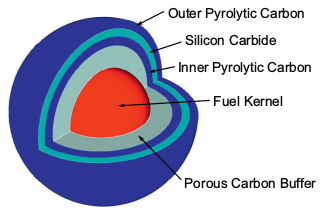
\includegraphics[height=3.5cm]{figures/triso}
	\caption{Drawing of a TRISO fuel particle. Image reproduced from \cite{hales_multidimensional_2013}.}
	\label{fig:triso}
\end{figure}

Another contributor to the passive safety of the \gls{HTGR} design is its materials.
Combining a graphite core structure, ceramic fuel, and inert helium permits exceedingly high operating temperatures \cite{ballinger_balance_2004}.
Graphite has a high heat capacity and maintains its strength at temperatures beyond 2760 $^{\circ}$C.
As a result, temperature changes in the core occur slowly and without damage to the core structure during transients.
The annular core geometry and low core power density also enable passive heat transfer mechanisms to remove the decay heat following postulated accidents \cite{neylan_modular_1988}.
These passive heat transfer mechanisms rely primarily on the natural processes of conduction, thermal radiation, and convection.

% Co-generation applications
A desirable feature of the \gls{HTGR} is its higher operating temperature.
Higher temperatures offer increased cycle efficiencies.
The early \gls{HTGR} designs converted their heat into electricity using the Rankine steam cycle \cite{herranz_power_2009}.
In such a system, the helium coolant passes through a heat exchanger generating steam to drive a  turbine.
This arrangement is around 38\% efficient \cite{breeze_nuclear_2014}.
Some of these designs would superheat the steam to increase their efficiency, but this complicates the plant layout \cite{ballinger_balance_2004}.
A practical temperature limit is around 300-400 $^{\circ}$C.
To take advantage of the high core outlet temperature of the \gls{HTGR}, the Brayton cycle is a better option because the helium coolant can directly drive a gas turbine in a closed cycle.
With such configuration, the system can achieve an energy conversion efficiency of around 48\% \cite{breeze_nuclear_2014}.
Additionally, having helium circulating in a closed cycle removes external sources of contamination of the nuclear circuit.
This reduces the need for on-line cleanup systems \cite{iaea_current_2001}.

Higher outlet temperatures and increased cycle efficiencies in HTGRs enable a wide range of process heat applications.
Some applications use steam for coal gasification processes, oil refinery processes, and production of synthesis gas, methanol, and hydrogen.
Hydrogen can be a decisive response to energy and climate challenges, as it can decarbonize the transport and power sectors \cite{nagashima_japans_2018}.
Several hydrogen production processes benefit from high temperatures, such as high-temperature electrolysis or thermochemical water splitting.
Utilizing the \gls{HTGR} as the energy source of the process eliminates the need to burn fossil fuels to generate the steam those processes require \cite{iaea_current_2001}.

% Maybe this paragraph should be in objectives
This thesis focuses primarily on the \gls{MHTGR}-350 \cite{neylan_modular_1988} \cite{silady_licensing_1988}.
Under the sponsorship of the \gls{US} \gls{DOE}, a team consisting of General Atomics, Combustion Engineering, General Electric, Bechtel National, Stone \& Webster Engineering, and \gls{ORNL} developed the \gls{MHTGR} \cite{neylan_modular_1988}.
They designed the basic module to deliver superheated steam at 17.3 MPa and 538 $^{\circ}$C.
Based on both economic and technological considerations, a 350 MWt modular reactor defines the optimal configuration.
The team completed in 1986 the preliminary safety information document for the \gls{MHTGR} and the complete draft pre-application in 1989 \cite{huning_steady_2014}.


\section{Motivation}

This work's ultimate goal is to support the development of \gls{HTGR} technology.
More specifically, we focus on the development of computational methods for modeling \glspl{HTGR} with \textit{Moltres} as our primary analysis tool.

% Why do we focus on HTGRs?
The Generation IV Roadmap project identified reactor concepts that could meet the future's energy demands in an efficient, economical, and environmentally safe manner \cite{macdonald_ngnp_2003}.
One of these reactor concepts is the \gls{VHTR}.
The \gls{VHTR} is distinct from the \gls{HTGR} as its coolant outlet temperature reaches higher temperatures.
However, the literature often uses these terms interchangeably.
In this work, the term \gls{HTGR} encompasses both terms.
The \gls{DOE} selected this reactor concept for the \gls{NGNP} Project.
This project intended to demonstrate emissions-free nuclear-assisted electricity and hydrogen production by 2015.

Although the \gls{DOE} canceled the \gls{NGNP} Project, \glspl{HTGR} may become a reality in the near term.
Some microreactor designs embody this type of technology and may be operational before 2030.
Additionally, as Section \ref{sec:pmr} has already described, the \gls{HTGR} technology has several favorable characteristics.
To recapitulate the most relevant features, the \gls{HTGR} relies on passive heat transfer mechanisms, uses TRISO particles as its fuel which inhibits proliferation, achieves high temperatures, and benefits from increased cycle efficiencies.
Another beneficial characteristic is that high temperatures enable a wide range of process heat applications, among which we find hydrogen production.

%Why is computational modeling important?
Modeling and prediction of core thermal-hydraulic behavior is necessary for assessing the safety characteristics of a reactor.
Determining the temperature inside a reactor, for both normal and transient operation, is of paramount importance as several materials' integrity depends on it.
Undesirably high temperatures endanger the TRISO particles' integrity and, consequently, jeopardize a fission product release \cite{tak_numerical_2008}.
% The temperatures in the core have to be kept below values that begin to cause damage to fission product barriers, produce stmctural material weakness, and lead to excessive chemical reaction rates.
Furthermore, the fuel blocks' complex geometry hinders accurate calculations of the fuel temperatures requiring elaborate numerical calculations.

The characteristics of an \gls{HTGR} are different from those of conventional \glspl{LWR}.
Such differences demand for new reactor analysis tools.
These new tools should take into account the following peculiarities of \glspl{HTGR} \cite{rohde_development_2012}\cite{bostelmann_criticality_2016}:
\begin{itemize}
\item Hexagonal structure: the shape of the fuel blocks hinders conformity to any orthogonal coordinate system.
\item Double heterogeneity: the TRISO particles form the first heterogeneity level, consisting of four
layers.
The second level arises from the fuel elements, as they encompass the compacts, the coolant, and the moderator.
\item Strong temperature dependence: the fuel temperatures have a large effect on the neutron spectrum and the macroscopic cross-sections.
\item High thermal inertia: the large graphite structures cause long transients.
\end{itemize}

%Why use Moltres?
Historically, linking a stand-alone neutronics solver to a thermal-hydraulics solver allowed for simulating an entire reactor.
The coupling of the programs occurred in a black-box fashion, such that one code's output served as the other's input and vice versa.
This coupling technique is commonly known as the operator-splitting technique \cite{ragusa_consistent_2009}.
In such an approach, each individual physics isolates the action of the governing equations upon the variables.
Nonetheless, these physical models describe processes that rely heavily on the solution of one another's.
The neutron flux determines the power distribution, and the power distribution strongly influences the temperature field.
Due to the \gls{HTGR} strong temperature feedback, the temperature affects the neutron flux distribution in the core.
Because of a time-scale separation between the different phenomena, multiphysics transient simulations coupled via the operator-splitting approach may introduce significant numerical errors \cite{ragusa_consistent_2009} \cite{park_tightly_2010}.

\gls{MOOSE} \cite{gaston_moose_2009} is a computational framework targeted at solving fully coupled systems.
All the software built on the \gls{MOOSE} framework shares a joint code base.
These features facilitate relatively easy coupling between separate phenomena and allow for great flexibility, even with a large variance in time scales \cite{novak_pronghorn_2018}.
Additionally, all programs use \gls{MPI} for parallel communication and allow for deployment on massively-parallel cluster-computing platforms.

\textit{Moltres} \cite{lindsay_introduction_2018} is an open source, \gls{FEM} simulation code built within the \gls{MOOSE} framework.
\textit{Moltres} solves arbitrary-group neutron diffusion, precursor, and temperature governing equations.
All these characteristics make \textit{Moltres} suitable for solving the type of physical phenomena described above.

\section{Objectives}

% This thesis focuses on steady-state calculations and also intends to set a roadmap for the transient simulations.
As mentioned earlier, the ultimate goal of this work is to support the development of \gls{HTGR} technology.
The following list of main objectives expands on that goal.

\paragraph{Extend Moltres modeling capabilities to \glspl{HTGR}.}
Moltres is a multi-physics solver of \glspl{MSR}.
Enhancing Moltres will allow it to model \glspl{HTGR} as well.

\paragraph{Couple the different physics phenomena present in an HTGR.}
Moltres's current capabilities allow for solving some of the physics in the HTGR design.
Nevertheless, the solver needs to capture the inherent physics in an HTGR and adequately integrate them into the current capabilities.

\paragraph{Develop safety analysis capabilities in Moltres.}
Steady-state simulations help understand the fundamental behavior of an HTGR and, like transient simulations, assist in reactor design. 
Transient simulations also assess the reactor response in design basis events.

\paragraph{Understand \gls{HTGR} contribution to stopping climate change.}
HTGRs are an attractive technology due to attaining high temperatures.
With such high temperatures, the efficiency of hydrogen production increases.

\vskip 0.6cm
The main objectives are somewhat broad.
The following list presents secondary objectives which will lead to the fulfillment of the main objectives:

\paragraph{Predict neutronics.}
Moltres should have the ability to carry out eigenvalue calculations appropriately.
Additionally, Moltres should predict the flux shape and magnitude accurately, during steady-state and transient simulations.

\paragraph{Understand the impact of some simulation parameters.}
The underlying physics of \glspl{HTGR} differ from the physics of other reactors.
Consequently, the simulation results will be sensitive to different parameters from other reactor type simulations.
This work will focus on the energy group structure and its effects on the diffusion calculations.
We will also assess how such parameters affect the performance of the simulations. 

\paragraph{Calculate power distribution correctly.}
The value of an accurate neutronics behavior prediction lies in the accurate prediction of the power distribution.
The power distribution is the most influential parameter over the thermal-hydraulics as it determines the temperature profile in the reactor.

\paragraph{Predict temperature profile accurately.}
Undesirably high temperatures endanger the integrity of the TRISO particles.
Additionally, the temperature influences the neutronics.
Hence, an accurate neutronics calculation will be inaccurate without a correct thermal-hydraulics calculation and vice versa. 

\paragraph{Develop a hydrogen production calculation tool.}
High temperatures enable high-efficiency hydrogen production methods.
Most of them have different energy requirements and production rates.
We will develop a tool to determine such quantities.